\documentclass{ctexart}
\usepackage{EC}
\begin{document}
\section{硼及其化合物}
\subsection{单质硼和金属硼化物}
由于单质硼和硼化物(尤其是和金属形成的硼化物)的结构比较类似,因此我们在此处一起介绍.
\subsubsection{单质硼的制备}
通过还原含硼化合物的方法可以方便地制备得到\ce{B}单质.
\begin{center}
    \ce{3Mg + B2O3 -> 3MgO + 2B}\\
    \ce{2KBF4 + 6KCl ->T[熔融\ce{KCl/KF}][电解] 8KF + 2B + 3Cl2}\\
    \ce{2BBr3 + 3H2 -> 2B + 6HBr}\\
    \ce{B_nH_m ->T[加热] n B + $\dfrac{m}{2}$ H2}
\end{center}
通常得到的硼是无定形的,但是改变温度条件也可以得到各种晶型的硼单质.
\subsubsection{单质硼的结构}
各种单质硼都具有相当复杂的结构,这主要是\ce{B}本身的缺电子结构使其的成键较为复杂所致.不过,一般而言,各种单质硼总是由\ce{\{B12\}}多面体衍生而来.
\paragraph{正十二面体与正二十面体的画法}
清晰地表示复杂簇合物的立体结构是你应当掌握的技巧.我们在这里介绍两种最典型的高对称性多面体的画法.
\subparagraph{正十二面体的画法}
我们可以按照以下步骤绘制正十二面体.
\begin{enumerate}[label=$\mathit{Step\ \arabic*.}$,topsep=0pt,parsep=0pt,itemsep=0pt,partopsep=0pt,leftmargin=*]
    \item 画一个正五边形.
    \item 画一个相对步骤$\mathit{1}$中旋转$180^\circ$的大小相同的正五边形,注意透视关系.
    \item 沿步骤$\mathit{1}$和步骤$\mathit{2}$中的两个正五边形的所有$10$条外角平分线方向画出等长的线段.
    \item 顺次连接步骤$\mathit{3}$中产生的各个外围顶点.
\end{enumerate}
\begin{figure}[H]
    \centering
    \subfigure[$\mathit{Step\ 1.}$]{
        \begin{minipage}[b]{.23\linewidth}
            \centering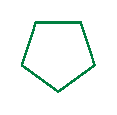
\includegraphics{picture/12-1.eps}
        \end{minipage}
    }
    \subfigure[$\mathit{Step\ 2.}$]{
        \begin{minipage}[b]{.23\linewidth}
            \centering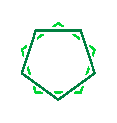
\includegraphics{picture/12-2.eps}
        \end{minipage}
    }
    \subfigure[$\mathit{Step\ 3.}$]{
        \begin{minipage}[b]{.23\linewidth}
            \centering
\includegraphics{picture/12-3.eps}
        \end{minipage}
    }
    \subfigure[$\mathit{Step\ 4.}$]{
        \begin{minipage}[b]{.23\linewidth}
            \centering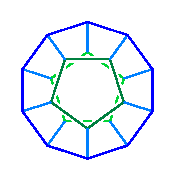
\includegraphics{picture/12-4.eps}
        \end{minipage}
    }
    \caption{正十二面体的画法}
\end{figure}
\subparagraph{正二十面体的画法}
我们可以按照以下步骤绘制正二十面体.
\begin{enumerate}[label=$\mathit{Step\ \arabic*.}$,topsep=0pt,parsep=0pt,itemsep=0pt,partopsep=0pt,leftmargin=*]
    \item 画一个正三角形(记为$\triangle{A}$).
    \item 画一个相对步骤$\mathit{1}$中旋转$180^\circ$的大小相同的正三角形(记为$\triangle{B}$),注意透视关系.
    \item 沿$\triangle{A}$和$\triangle{B}$的所有$6$条外角平分线画出等长的线段.
    \item 将$\triangle{B}$形成的外围顶点与$\triangle{A}$的顶点依次连接.
    \item 将$\triangle{A}$形成的外围顶点与$\triangle{B}$的顶点依次连接,注意透视关系.
    \item 顺次连接步骤$\mathit{3}$中产生的各个外围顶点.
\end{enumerate}
\begin{figure}[H]
    \centering
    \subfigure[$\mathit{Step\ 1.}$]{
        \begin{minipage}[b]{.3\linewidth}
            \centering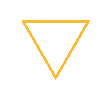
\includegraphics{picture/20-1.eps}
        \end{minipage}
    }
    \subfigure[$\mathit{Step\ 2.}$]{
        \begin{minipage}[b]{.3\linewidth}
            \centering
\includegraphics{picture/20-2.eps}
        \end{minipage}
    }
    \subfigure[$\mathit{Step\ 3.}$]{
        \begin{minipage}[b]{.3\linewidth}
            \centering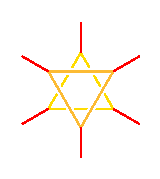
\includegraphics{picture/20-3.eps}
        \end{minipage}
    }
    \subfigure[$\mathit{Step\ 4.}$]{
        \begin{minipage}[b]{.3\linewidth}
            \centering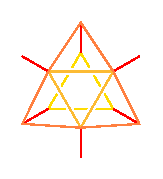
\includegraphics{picture/20-4.eps}
        \end{minipage}
    }
    \subfigure[$\mathit{Step\ 5.}$]{
        \begin{minipage}[b]{.3\linewidth}
            \centering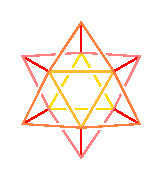
\includegraphics{picture/20-5.eps}
        \end{minipage}
    }
    \subfigure[$\mathit{Step\ 6.}$]{
        \begin{minipage}[b]{.3\linewidth}
            \centering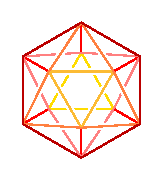
\includegraphics{picture/20-6.eps}
        \end{minipage}
    }
    \caption{正二十面体的画法}
\end{figure}
\paragraph{硼的同素异形体}
我们主要(简单地)介绍以下几种硼的同素异形体.
\begin{enumerate}[label=\tbf{\arabic*.},topsep=0pt,parsep=0pt,itemsep=0pt,partopsep=0pt]
    \item $\alpha$-三方硼\\
        $\alpha$-三方硼是硼最简单的同素异形体.它由近似立方密堆积的\ce{B12}二十面体组成,因而退化成R心六方点阵.
        \begin{figure}[H]
            \centering
            \subfigure[$\alpha$-三方硼的晶胞示意图]{
                \begin{minipage}[b]{.48\linewidth}
                    \centering\includegraphics[scale=0.1]{picture/alpha-B.eps}
                \end{minipage}
            }
            \subfigure[$\alpha$-三方硼沿$\mbf{a}+\mbf{b}$方向的投影图]{
                \begin{minipage}[b]{.48\linewidth}
                    \centering\includegraphics[scale=0.1]{picture/alpha-B-2.eps}
                \end{minipage}
            }
            \caption{$\alpha$-三方硼的晶体结构}
        \end{figure}
    \item $\beta$-三方硼\\
        $\beta$-三方硼是硼在热力学上最稳定的同素异形体.它的结构则要复杂得多.\\
        $\beta$-三方硼的晶胞中有$105$个\ce{B}原子.其中的\ce{B84}单元是由\ce{B12}二十面体以及每个\ce{B}相连的\ce{B6}单元组成.\ce{B6}单元是向外的五角锥形,与正二十面体的一部分几乎一致.\ce{B84}单元之间由\ce{B10}半二十面体(注意其结构类似二十面体的一部分)以及额外的一个\ce{B}原子连接,比例为$1:2:1$,因此结构基元总计有$105$个\ce{B}原子.
        \begin{figure}[H]
            \centering
            \subfigure[\ce{B84}单元的结构示意图]{
                \begin{minipage}[b]{.48\linewidth}
                    \centering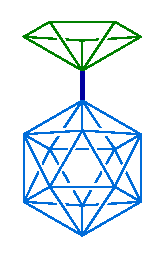
\includegraphics{picture/B84.eps}
                \end{minipage}
            }
            \subfigure[\ce{B10}单元的结构示意图]{
                \begin{minipage}[b]{.48\linewidth}
                    \centering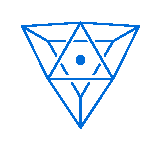
\includegraphics{picture/B10.eps}
                \end{minipage}
            }
            \caption{$\beta$-三方硼的结构示意图}
        \end{figure}
        至于整体的晶胞,因为太过复杂,故此处不单独展示.如果你有兴趣,可以自行查阅其晶胞\footnote{恕笔者直言,长得有点奇行种.}.
    \item 其它硼的同素异形体\\
        总而言之,其它硼的同素异形体,例如$\beta$-四方硼,$\gamma$-硼的结构都与上述两者有类似之处,都是由\ce{B12}二十面体及其衍生结构组成的.它们的晶胞也比较复杂,你可以自行查阅之.
\end{enumerate}
\subsubsection{金属硼化物的制备}
制备金属硼化物主要有以下几种方法.
\begin{enumerate}[label=\tbf{\arabic*.},topsep=0pt,parsep=0pt,itemsep=0pt,partopsep=0pt]
    \item 直接由单质直接化合.例如:
        \begin{center}
            \ce{Cr + n B ->T[$1150\tc$] CrB_n}
        \end{center}
    \item 用硼单质还原金属氧化物(这种办法比较浪费难得的硼单质).例如:
        \begin{center}
            \ce{Sc2O3 + 7B ->T[$1800\tc$] 2ScB2 + 3BO}
        \end{center}
        这里需要注意的是\ce{B}单质和\ce{B2O3}大约在$1350\tc$时反应生成玻璃状的\ce{(BO)_n}聚合物.
    \item 用\ce{H2}还原金属和硼的卤化物混合物,或用碳还原金属和硼的氧化物混合物,或用硼碳化物还原金属氧化物.例如:
        \begin{center}
            \ce{2TiCl4 + 4BCl3 + 10H2 ->T[$1300\tc$] 2TiB2 + 20HCl}\\
            \ce{V2O5 + B2O3 + 8C ->T[$1500\tc$] 2VB + 8CO}\\
            \ce{Eu2O3 + 3B4C ->T[$1600\tc$] 2EuB6 + 3CO}\\
            \ce{7Ti + B2O3 + 3B4C ->T[$2000\tc$] 7TiB2 + 3CO}
        \end{center}
    \item 熔融盐的电解沉积.将金属氧化物和\ce{B2O3}混合熔融于合适的盐中,然后用石墨电极电解即可在阴极得到硼化物.
\end{enumerate}
\subsubsection{金属硼化物的结构}
\paragraph{富金属的金属硼化物}
这类物质的通式为\ce{M_n B},其中\ce{M}为金属元素并且(大致而言)$n\geqslant0.5$.通常而言,硼原子总是处于三棱柱(或者加数个帽)的配位环境中,并且随着$n$变小时,\ce{B}还会从分立转为线形的\ce{B2},链状或平面的\ce{B_n}等形式.\\
\indent 这里给出一些简单的例子以供参考.
\begin{figure}[H]
    \centering
    \subfigure[\ce{MgB2}的晶胞示意图]{
        \begin{minipage}[b]{.48\linewidth}
            \centering\includegraphics[scale=0.1]{picture/MgB2-1.eps}
        \end{minipage}
    }
    \subfigure[\ce{MgB2}的$c$轴投影图]{
        \begin{minipage}[b]{.48\linewidth}
            \centering\includegraphics[scale=0.1]{picture/MgB2-2.eps}
        \end{minipage}
    }
    \caption{\ce{MgB2}的晶体结构}
\end{figure}
\begin{figure}[H]
    \centering
    \subfigure[\ce{ReB3}的晶胞示意图]{
        \begin{minipage}[b]{.48\linewidth}
            \centering\includegraphics[scale=0.1]{picture/Re3B-1.eps}
        \end{minipage}
    }
    \subfigure[\ce{ReB3}的晶胞示意图]{
        \begin{minipage}[b]{.48\linewidth}
            \centering\includegraphics[scale=0.1]{picture/Re3B-2.eps}
        \end{minipage}
    }
    \caption{\ce{ReB3}的晶体结构}
\end{figure}
\paragraph{富硼的金属硼化物}
富硼的金属硼化物,从\ce{MB4}到\ce{MB66}等等,大多以\ce{B}的团簇和填充其中的金属原子组成.我们现在选取主要的几种进行介绍.
\begin{enumerate}[label=\tbf{\arabic*.},topsep=0pt,parsep=0pt,itemsep=0pt,partopsep=0pt]
    \item \tbf{\ce{MB4}}\\
        典型的如四方晶系的\ce{ThB4},其中含有\ce{B6}八面体结构,并由线形的\ce{B2}在层内将其相连;\ce{Th}原子则填充在它们形成的$c$轴方向的空隙中.对于\ce{B2}单元中的\ce{B}原子,仍然被\ce{Th}原子六配位.这可以视作\ce{MB2}和\ce{MB6}结构中间的过渡.
        \begin{figure}[H]
            \centering
            \subfigure[\ce{ThB4}的晶胞示意图]{
                \begin{minipage}[b]{.48\linewidth}
                    \centering\includegraphics[scale=0.1]{picture/ThB4-1.eps}
                \end{minipage}
            }
            \subfigure[\ce{ThB4}的晶胞示意图]{
                \begin{minipage}[b]{.48\linewidth}
                    \centering\includegraphics[scale=0.1]{picture/ThB4-2.eps}
                \end{minipage}
            }
            \caption{\ce{ThB4}的晶体结构}
        \end{figure}
    \item \tbf{\ce{B4C}}\\
        确切的验证表明实际上组成为\ce{B13C2},但是也可以在\ce{B13C2}到\ce{B12C3}(即\ce{B4C})的范围内变动.\ce{B13C2}的晶体结构如下所示.
        \begin{figure}[H]
            \centering
            \subfigure[\ce{B13C2}的晶胞示意图]{
                \begin{minipage}[b]{.48\linewidth}
                    \centering\includegraphics[scale=0.1]{picture/B13C2-1.eps}
                \end{minipage}
            }
            \subfigure[\ce{B13C2}的晶胞示意图]{
                \begin{minipage}[b]{.48\linewidth}
                    \centering\includegraphics[scale=0.1]{picture/B13C2-2.eps}
                \end{minipage}
            }
            \caption{\ce{B13C2}的晶体结构}
        \end{figure}
        \indent 这种三方晶系的晶体可以视作线形\ce{CBC}单元做立方密堆积,\ce{B12}单元填入所有八面体空隙中而形成的.把\ce{CBC}单元中的\ce{B}也(部分地)换成\ce{C},就可以得到组成逐渐接近\ce{B4C}的物质.
    \item \tbf{\ce{MB6}}\\
        典型的如立方晶系的\ce{LaB6}.其中的\ce{B6}八面体单元按简单立方堆积形成网状结构,\ce{La}则填入所有立方体空隙中.因此,\ce{La}原子的配位数为$24$,配位多面体为截角立方体,每个与其相邻的\ce{B6}八面体贡献一个三角形面.
        \begin{figure}[H]
            \centering
            \subfigure[\ce{LaB6}的晶胞示意图]{
                \begin{minipage}[b]{.48\linewidth}
                    \centering\includegraphics[scale=0.1]{picture/LaB6-1.eps}
                \end{minipage}
            }
            \subfigure[\ce{LaB6}的八倍晶胞示意图]{
                \begin{minipage}[b]{.48\linewidth}
                    \centering\includegraphics[scale=0.1]{picture/LaB6-2.eps}
                \end{minipage}
            }
            \subfigure[\ce{LaB6}中\ce{La}的配位多面体]{
                \begin{minipage}[b]{.9\linewidth}
                    \centering\includegraphics[scale=0.1]{picture/LaB6-3.eps}
                \end{minipage}
            }
            \caption{\ce{LaB6}的晶体结构}
        \end{figure}
    \item \tbf{\ce{MB12}}\\
        典型的如立方晶系的\ce{UB12}.其中的\ce{B12}单元并不是常见的正二十面体,而是立方八面体.你可以将立方体的棱心依次连接而得到它的形状.\\
        在\ce{UB12}中,\ce{B12}立方八面体做立方密堆积,\ce{U}原子填入所有八面体空隙.其中的\ce{U}原子也是$24$配位的,但配位形式是截角八面体,每个与其相邻的\ce{B12}单元贡献一个正方形面.\\
        顺带一提,此时\ce{B12}单元形成的四面体空隙是一个截角四面体,每个\ce{B12}立方八面体贡献一个三角形面.
        \begin{figure}[H]
            \centering
            \subfigure[\ce{UB12}的晶胞示意图]{
                \begin{minipage}[b]{.48\linewidth}
                    \centering\includegraphics[scale=0.1]{picture/UB12-1.eps}
                \end{minipage}
            }
            \subfigure[\ce{UB12}晶胞的$a$轴投影图]{
                \begin{minipage}[b]{.48\linewidth}
                    \centering\includegraphics[scale=0.1]{picture/UB12-2.eps}
                \end{minipage}
            }
            \caption{\ce{UB12}的晶体结构}
        \end{figure}
\end{enumerate}
\subsection{硼烷及其衍生物}
\subsubsection{Wade规则}
\paragraph{Wade规则介绍}
多面体骨架电子对理论(Polyhedral Skeletal Electron Pair Theory, PSEPT)试图从多面体骨架的几何形状和电子数之间的关系上来阐明金属原子簇的结构规律.这一规则最初由Kenneth Wade制定,因此又被称为Wade规则.\\
\indent 我们现在来介绍Wade规则的具体内容.\\
\indent $\mathit{Step\ 1.}$\ \tbf{确定骨架原子数}\\
\indent 骨架原子通常是IVA族及之前的元素或过渡金属元素,而\ce{N,O}等元素则应当作为额外的配体考虑.这样就能确定骨架原子数$n$.\\
\indent $\mathit{Step\ 2.}$\ \tbf{确定骨架电子数}\\
\indent 每个骨架原子都拿出三个价轨道参与骨架的成键,剩余的价轨道一般对应端基原子且需要填满.在满足端基的情况下,骨架原子剩余的电子参与成键,将计入骨架电子数.\\
\indent 例如,对于硼烷而言,骨架\ce{B}原子有四个价轨道,除去三个用于构成骨架之外剩余一个与端基\ce{H}相连,端基\ce{B-H}键需用去\ce{B}的一个价电子,因而剩余$2$个电子计入骨架电子数.类似地,对于碳硼烷中的\ce{CH}基团而言,将有$3$个电子计入骨架电子数.\\
\indent 对于过渡金属\ce{M}的羰基簇合物而言,\ce{M}有九个价轨道,除去三个用于构成骨架之外剩余六个价轨道.假设其价电子数为$v$,端基配位的基团提供的总电子数为$w$,那么充满六个价轨道后计入骨架电子的数目为$v+w-12$.下面是一些典型的过渡金属碎片提供的骨架电子数.
\begin{table}[H]
    \centering
    \begin{tabular}{c|c|c|c|c|c}
        \hline
        $v$ &过渡金属\ce{M} &\ce{M(CO)2}$(w=4)$ &\ce{M(Cp)}$(w=5)$  &\ce{M(CO)3}$(w=6)$ &\ce{M(CO)4}$(w=8)$ \\\hline
        $6$ &\ce{Cr,Mo,W}   &$-$    &$-1$   &$0$    &$2$ \\
        $7$ &\ce{Mn,Tc,Re}   &$-1$    &$0$   &$1$    &$3$ \\
        $8$ &\ce{Fe,Ru,Os}   &$0$    &$1$   &$2$    &$4$ \\
        $9$ &\ce{Co,Rh,Ir}   &$1$    &$2$   &$3$    &$-$ \\
        $10$ &\ce{Ni,Pd,Pt}   &$2$    &$3$   &$-$    &$-$ \\\hline
    \end{tabular}
    \caption{过渡金属碎片提供的骨架电子数}
\end{table}
从这里可以看出,\ce{Fe(CO)3}等基团提供的电子数与\ce{BH}相同,\ce{Co(CO)3}等基团提供的电子数与\ce{CH}相同.事实上,在大部分化合物中,这些基团可以相互替换,表现出了相似的性质.这就是\tbf{等瓣相似原理}.\\
\indent 除此之外,尚有不是端基的一些配体.它们通常作为桥连配体或存在于骨架内部,依照不同的配位方式提供不同的电子数目,并全部计入骨架电子数目中.例如,\ce{H}原子计$1$个电子,\ce{CO}配体计$2$个电子,边桥基的\ce{O}原子计$2$个电子,面桥基和体内则分别计$4$个和$6$个电子,等等.\\
\indent 最后,如果我们考虑的对象是离子,应将电荷也计入骨架电子中.\\
\indent 按照以上的步骤,我们就能得出骨架电子数$m$.\\
\indent $\mathit{Step\ 3.}$\ \tbf{确定骨架的结构}\\
\indent Wade发现$m$和$n$之间的关系决定了簇合物的立体结构.简单而言,\tbf{簇合物是由$\dfrac{m}{2}-1$个顶点的闭式多面体去掉$\dfrac{m}{2}-n-1$个顶点形成的多面体}.\\
\indent 上面这句话听起来很拗口.我们首先来解决第一个问题:闭式多面体的定义.简而言之,闭式多面体是全部由三角形面构成的闭合的多面体.具有$N$个顶点的闭式多面体展示如下.
\begin{figure}[H]
    \centering
    \subfigure[$N=4$\ 正四面体]{\begin{minipage}[b]{.3\linewidth}\centering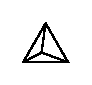
\includegraphics{picture/closo-4.eps}\end{minipage}}
    \subfigure[$N=5$\ 三角双锥]{\begin{minipage}[b]{.3\linewidth}\centering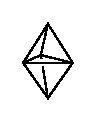
\includegraphics{picture/closo-5.eps}\end{minipage}}
    \subfigure[$N=6$\ 正八面体]{\begin{minipage}[b]{.3\linewidth}\centering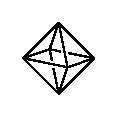
\includegraphics{picture/closo-6.eps}\end{minipage}}
    \subfigure[$N=7$\ 五角双锥]{\begin{minipage}[b]{.3\linewidth}\centering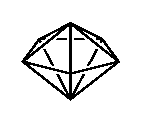
\includegraphics{picture/closo-7.eps}\end{minipage}}
    \subfigure[$N=8$\ 三角十二面体]{\begin{minipage}[b]{.3\linewidth}\centering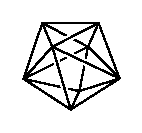
\includegraphics{picture/closo-8.eps}\end{minipage}}
    \subfigure[$N=9$\ 三帽三棱柱]{\begin{minipage}[b]{.3\linewidth}\centering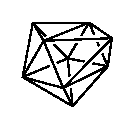
\includegraphics{picture/closo-9.eps}\end{minipage}}
    \subfigure[$N=10$\ 双帽四方反棱柱]{\begin{minipage}[b]{.3\linewidth}\centering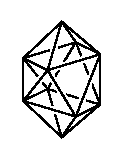
\includegraphics{picture/closo-10.eps}\end{minipage}}
    \subfigure[$N=11$\ 边收缩二十面体]{\begin{minipage}[b]{.3\linewidth}\centering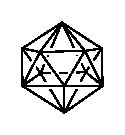
\includegraphics{picture/closo-11.eps}\end{minipage}}
    \subfigure[$N=12$\ 正二十面体]{\begin{minipage}[b]{.3\linewidth}\centering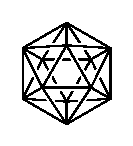
\includegraphics{picture/closo-12.eps}\end{minipage}}
    \caption{具有$N$个顶点的闭式多面体}
\end{figure}
现在,我们按照去除顶点的个数对簇合物分类.
\begin{table}[H]
    \centering\begin{tabular}{|c|c|c|c|}
        \hline
        $m$的取值   &中文名称   &拉丁文名称 &形状\\\hline
        $2n-2$  &双帽闭式   &Bicapped\ $\mathit{closo}$ & 双加帽的具有$n-2$个顶点的闭式多面体 \\\hline
        $2n$  &单帽闭式   &Capped\ $\mathit{closo}$ & 加帽的具有$n-1$个顶点的闭式多面体 \\\hline
        $2n+2$  &闭式   &$\mathit{closo}$ & 具有$n$个顶点的闭式多面体 \\\hline
        $2n+4$  &巢式   &$\mathit{nido}$ & 具有$n+1$个顶点的闭式多面体去除$1$个顶点 \\\hline
        $2n+6$  &蛛网式   &$\mathit{arachno}$ & 具有$n+2$个顶点的闭式多面体去除$2$个顶点 \\\hline
        $2n+8$  &开式   &$\mathit{hypho}$ & 具有$n+3$个顶点的闭式多面体去除$3$个顶点 \\\hline
    \end{tabular}
    \caption{簇合物骨架形状与$m$和$n$的关系}
\end{table}
下面这张图\footnote{https://en.wikipedia.org/wiki/File:Deltahedral-borane-cluster-array-numbered-3D-bs-17.png.}给出了典型的结构\footnote{限于排版原因,请将讲义顺时针旋转$90^\circ$后查阅此图.}.
\begin{figure}[H]
    \centering\includegraphics[scale=0.06,angle=90]{picture/Wade.eps}\caption{Wade规则所预测的多面体形状}
\end{figure}
\indent $\mathit{Step\ 4.}$\ \tbf{确定非端基配体的位置}\\
\indent 实际上端基配体的位置是比较难以确定的.很多配体的不同配位形式所提供的电子数目一致.因此,在没有额外条件下,你可以尽量猜测研究对象具有较高的对称性.
\paragraph{Wade规则的简单应用}
我们在本节举几个简单的例子来说明Wade规则如何应用.\\
$\mathit{Example\ 1.}$\ \ce{[B6H6]^2-}\\
\indent 骨架原子数$n=6$,骨架电子数$m=6\times2+2=14$,因此$m=2n+2$,采取顶点数$N=6$的正八面体结构,无需增删顶点.
\chemfig{B6H62-}{1}{\ce{[B6H6]^2-}的结构}
类似地,你可以知道\ce{[B_nH_n]^2-}的结构就是顶点数$N=n$的闭式多面体.\\
$\mathit{Example\ 2.}$\ \ce{B10C2H12}\\
\indent 骨架原子数$n=12$,骨架电子数$m=10\times2+2\times3=26$,因此$m=2n+2$,采取顶点数$N=12$的正二十面体结构,无需增删顶点.由于\ce{C}原子相对位置的不同,\ce{B10C2H12}事实上有三种异构体.\vspace{-5pt}
\begin{figure}[H]
    \centering
    \subfigure[$o$-\ce{B10C2H12}]{
        \begin{minipage}[b]{.3\linewidth}
            \centering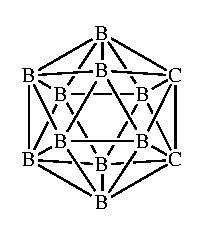
\includegraphics{picture/B10C2H12-o.eps}
        \end{minipage}
    }
    \subfigure[$m$-\ce{B10C2H12}]{
        \begin{minipage}[b]{.3\linewidth}
            \centering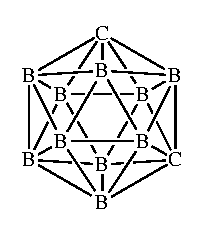
\includegraphics{picture/B10C2H12-m.eps}
        \end{minipage}
    }
    \subfigure[$p$-\ce{B10C2H12}]{
        \begin{minipage}[b]{.3\linewidth}
            \centering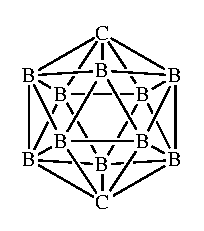
\includegraphics{picture/B10C2H12-p.eps}
        \end{minipage}
    }
    \caption{\ce{B10C2H12}的异构体的结构(省略所有端基\ce{H}原子)}
\end{figure}\vspace{-10pt}
类似地,你也可以知道\ce{B_{n-2}C2H_n}的结构就是顶点数$N=n$的闭式多面体(不考虑键长差异带来的轻微畸变).
$\mathit{Example\ 3.}$\ \ce{B6H10}\\
\indent 骨架原子数$n=6$,骨架电子数$m=6\times2+4\times1=16$,因此$m=2n+4$,采取顶点数$N=7$的五角双锥结构并删去一个顶点.它的投影图和平面结构如下所示.\vspace{-10pt}
\begin{figure}[H]
    \centering
    \subfigure[\ce{B6H10}的立体结构示意图]{
        \begin{minipage}[b]{.45\linewidth}
            \centering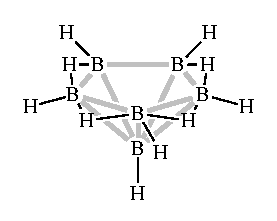
\includegraphics{picture/B6H10-1.eps}
        \end{minipage}
    }
    \subfigure[\ce{B6H10}的成键方式示意图]{
        \begin{minipage}[b]{.45\linewidth}
            \centering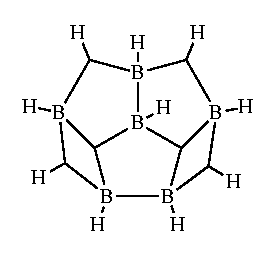
\includegraphics[scale=0.9]{picture/B6H10-2.eps}
        \end{minipage}
    }\caption{\ce{B6H10}的结构}
\end{figure}
事实上,\ce{B6H10}就是典型的巢式硼烷.\\
$\mathit{Example\ 4.}$\ \ce{Os7(CO)21}\\
\indent 骨架原子数$n=7$,骨架电子数$m=7\times(8+3\times2-12)=14$,因此$m=2n$,采取顶点数$N=6$的八面体结构并加一个帽.事实上,这一羰基簇合物就是单加帽八面体形的.你可以自己尝试绘出其结构.\\
$\mathit{Example\ 5.}$\ \ce{Fe5(CO)15C}\\
\indent 骨架原子数$n=5$,骨架电子数$m=5\times(8+3\times2-12)+4=14$,因此$m=2n+4$,采取顶点数$N=6$的八面体结构并删去一个顶点.事实上,这一羰基簇合物就是四棱锥形的,\ce{C}原子位于棱锥中心.你可以自己尝试绘出其结构.\\
$\mathit{Example\ 6.}$\ \ce{[Pb9]^4-}\\
\indent 骨架原子数$n=9$,骨架电子数$m=9\times2+4=22$,因此$m=2n+4$,采取顶点数$N=10$的双帽四方反棱柱结构并删去一个顶点.事实上,\ce{[Pb9]^4-}和\ce{[Sn9]^4-}都是单帽四方反棱柱形的.
\chemfig{M94-}{1}{\ce{[M9]^4-}(\ce{M=Pb,Sn})的结构}
$\mathit{Example\ 7.}$\ \ce{[Bi8]^2+}\\
\indent 骨架原子数$n=8$,骨架电子数$m=8\times3-2=22$,因此$m=2n+6$,采取顶点数$N=10$的双帽四方反棱柱结构并删去两个顶点.我们在之前就已经讲过这一离子是四方反棱柱的,这也符合Wade规则所预测的结果.
\paragraph{Wade规则的局限性}
尽管对于简单的簇合物而言,Wade规则总是正确的,然而对于稍显奇怪的物质就不那么准确了.首先,Wade规则无法预测具有单电子的簇合物,而它们通常具有与预测结构相不同的形状.其次,对于某些元素,例如\ce{Rh}的多核团簇而言,预期的结构也与Wade规则有所差别.\\
\indent 确切而言,使用Wade规则的最佳场景是解释某簇合物的结构,而在预测结构时则由于配体配位形式的不同使得骨架电子数不同等情况而使结果具有一定的任意性.不过大部分时候,簇合物总是符合Wade规则的(或者你可以将它解释地符合Wade规则).如果你在做题时有闲心,也可以验证一下你的答案是否符合Wade规则,但这仅仅作为参考,并不能作为决定结构正确与否的绝对依据.
\subsubsection{价键理论对硼烷成键形式的解释与$styx$码}
\paragraph{三中心二电子键}
由于\ce{B}元素的缺电子性质,成键时为了满足八电子,时常需要形成非经典的$\sigma$键(IIA和IIIA族的元素经常如此).我们以最简单的硼烷\ce{B2H6}为例介绍硼烷中的成键方式.\\
\indent 想象\footnote{这一段内容只是对\ce{B2H6}成键方式的一种形象地推理,并不具备严格的学术参考价值.}(理论上)最简单的硼氢化物\ce{BH3}.其中的\ce{B}原子并不满足八隅律,因而期望从别的地方再找一对电子来.能找到的自然只有$\sigma\left(\ce{B-H}\right)$电子,因此两个\ce{BH3}决定互相共用这一对电子,从而满足八隅律,使得结构稳定.\\
\indent 对于这个共用的电子,两个\ce{B}各提供一个$\text{sp}^3$轨道,一个\ce{H}提供$\text{s}$轨道,组合形成新的轨道后在最低的能级填入两个电子.这就是\ce{B2H6}中的三中心二电子键的由来.
\chemfig{3c2e}{0.25}{\ce{BHB}三中心二电子键的轨道组合方式示意图}
我们可以把三中心二电子键画成三个原子各伸出一根短键后交汇于一点的形式.这样,\ce{B2H6}就能画成如下形式:
\chemfig{B2H6}{1}{\ce{B2H6}的结构}
另一种三中心二电子键是\ce{BBB}三中心二电子键.它与\ce{BHB}三中心二电子键几乎一致,除了参与组合的三个轨道均为\ce{B}的$\text{sp}^3$轨道.
\paragraph{$styx$规则}
在硼烷中,价电子的总数不能满足每两个相邻原子都以常规的$\sigma$键结合,因而需要形成三中心二电子键.成键的情况可以用$styx$数码表示.\\
\indent $styx$数码分别表示\ce{BHB}三中心二电子键$(s)$,\ce{BBB}三中心二电子键$(t)$,\ce{B-B}单键$(y)$和\ce{BH2}基团$(x)$的数目.用价键理论描述硼烷的成键方式时需满足如下规则:
\begin{enumerate}[label=\tbf{\arabic*.},topsep=0pt,parsep=0pt,itemsep=0pt,partopsep=0pt]
    \item 相邻的\ce{B}原子均由\ce{BHB},\ce{BBB}或\ce{B-B}键连接.
    \item 每个\ce{B}原子均用其四个价轨道成键,达到八电子组态.
    \item 如果相邻的\ce{B}原子已经成\ce{B-B}键,那么就不能再成\ce{BHB}或\ce{BBB}键.
    \item 每个\ce{B}原子至少与一个端基\ce{H}原子相连.
\end{enumerate}
遵照以上规则,我们可以对于化学式为\ce{B_nH_m}的硼烷列出以下方程:
\[\left\{\begin{array}{l}
    s+x=m-n\\
    3n+m=2(n+s+t+y+x)\\
    4n+m=2n+3(s+t)+2(x+y)
\end{array}\right.\]
这三个等式分别对应\ce{H}原子守恒,电子守恒和轨道数目守恒.此外,还需满足$s,t,y,x$均为非负整数这一条件.对于部分简单硼烷而言,上述方程组都有唯一解,可以根据对应的数码轻松地画出其结构.然而,也有很多硼烷对应了多种解\footnote{例如\ce{B5H9}一共有$4120,3211,2302$三种解.}.这就需要根据规则\tbf{3}对结构进行排除.下面给出了一些硼烷的结构与对应的$styx$数码.
\begin{figure}[H]
    \centering
    \subfigure[\ce{B2H6}\ $2002$]{\begin{minipage}[b]{.3\linewidth}\centering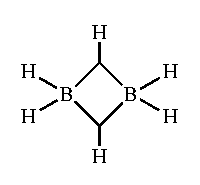
\includegraphics{picture/B2H6-1.eps}\end{minipage}}
    \subfigure[\ce{B4H10}\ $4012$]{\begin{minipage}[b]{.3\linewidth}\centering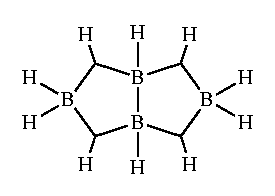
\includegraphics{picture/B4H10.eps}\end{minipage}}
    \subfigure[\ce{B5H9}\ $4120$]{\begin{minipage}[b]{.3\linewidth}\centering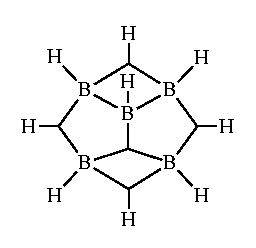
\includegraphics{picture/B5H9.eps}\end{minipage}}
    \subfigure[\ce{B6H10}\ $4220$]{\begin{minipage}[b]{.3\linewidth}\centering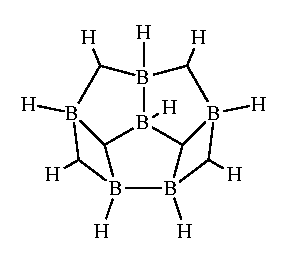
\includegraphics{picture/B6H10.eps}\end{minipage}}
    \subfigure[\ce{B7H15}\ $6122$]{\begin{minipage}[b]{.4\linewidth}\centering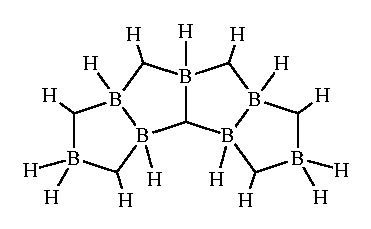
\includegraphics{picture/B7H15.eps}\end{minipage}}
    \caption{几种简单硼烷的结构及其$styx$数码}
\end{figure}
\subsubsection{硼烷和硼氢化物的化学性质}
\paragraph{硼烷的性质概述}
硼烷是无色的,抗磁性的,热稳性不高的化合物.低级硼烷在室温下为气体,但随着分子量增加而变成挥发性的液体或固体.硼烷的生成都是吸热的,但这并不是因为\ce{B-H}键弱的缘故,而是硼单质和\ce{H2}中的\ce{B-B}键和\ce{H-H}键较强的缘故.\\
\indent 硼烷的化学性质是活泼的,它们大多具有明显的还原性.一些硼烷在空气中即可发生自燃.一般而言,随着结构越偏离闭式,硼烷就越不稳定,而闭式的\ce{[B_nH_n]^2-}则是相当稳定的.
\paragraph{\ce{BH4-}及其盐的性质}
我们先从此系列最简单的离子,\ce{BH4-}开始讲起.显然地,作为\ce{CH4}的等电子体,这是一种呈现正四面体构型的离子.
\chemfig{BH4-}{1}{\ce{BH4-}离子的结构示意图}
硼烷化学的发展得益于第二次世界大战,当时美国国防部在寻找一种分子量尽量小的挥发性铀化合物用于裂变材料\ce{^235U}的富集,而\ce{U(BH4)4}符合这个要求.合成\ce{U(BH4)4}需要用到\ce{LiH},然而\ce{LiH}的供应很少,于是就用便宜的\ce{NaH}代替,而\ce{NaBH4}就在这个过程中被发现\footnote{后来,因为\ce{UF6}的处理工艺问题得到解决,他们便放弃了通过\ce{U(BH4)4}来富集\ce{^235U}的计划,而研究课题就变成了如何方便地制备\ce{NaBH4}.}.
\begin{substance}[\ce{NaBH4}]
    硼氢化钠,化学式为\ce{NaBH4},是一种白色的,易吸水潮解的白色粉末,可溶于水和低级醇,有一定的毒性.
\end{substance}
\indent 通常,可以通过下面的方法制备或生产\ce{NaBH4}.
\begin{center}
    \ce{4NaH + B(OCH3)3 -> NaBH4 + 3NaOCH3}\\
    \ce{Na2B4O7 + 16Na + 8H2 + 7SiO2 -> 4NaBH4 + 7Na2SiO3}\\
    \ce{NaBO2 + 4Na + 2H2 + 2SiO2 -> NaBH4 + 2Na2SiO3}
\end{center}
\indent \ce{NaBH4}经常被用作还原剂(还原产物通常都是\ce{NaB(OH)4},尤其是在水溶液中.).它可以将\ce{SO2}还原为\ce{S2O4^2-}:
\begin{center}
    \ce{NaBH4 + 8NaOH + 8SO2 -> 4Na2S2O4 + NaB(OH)4 + 4H2O}
\end{center}
也可以用于给非金属材料上镀镍\footnote{这个反应的方程式确乎令人迷惑,不必太过在意.}:
\begin{center}
    \ce{20NiCl2 + 16NaBH4 + 34NaOH + 6H2O -> 6Ni3B + 2Ni + 10NaB(OH)4 + 40NaCl + 35H2}
\end{center}
在有机化学中,\ce{NaBH4}被经常地用于还原羰基化合物.具体的选择性在各类有机化学书中都有介绍,在这里就不再详细说明.总而言之,相比\ce{LiAlH4}等还原剂而言,\ce{NaBH4}是相对温和的,选择性也相对高的一种还原剂.\\
\indent \ce{BH4-}与卤化物反应的产物主要取决于元素的电正性.对于大部分主族金属元素,镧系元素和钛分族等电正性较强的元素,总是倾向得到硼氢化物\ce{M(BH4)_n}.而对于大部分过渡金属元素和主族非金属元素则得到氢化物与\ce{H-}配合物为主.\\
\indent \ce{BH4-}可以作为$\eta^1,\eta^2$和$\eta^3$配体进行配位.$\eta^3$配位的典型例子是\ce{Zr(BH4)4},其中\ce{Zr}原子的配位形式是略微变形的截角立方体.
\begin{figure}[H]
    \centering
    \subfigure[\ce{Zr(BH4)4}的晶胞示意图]{
        \begin{minipage}[b]{.48\linewidth}
            \centering\includegraphics[scale=0.1]{picture/Zr(BH4)4-1.eps}
        \end{minipage}
    }
    \subfigure[\ce{Zr(BH4)4}的晶胞沿对角线的投影图]{
        \begin{minipage}[b]{.48\linewidth}
            \centering\includegraphics[scale=0.1]{picture/Zr(BH4)4-2.eps}
        \end{minipage}
    }
    \caption{\ce{Zr(BH4)4}的晶体结构}
\end{figure}
\paragraph{乙硼烷\ce{B2H6}的性质}
\subparagraph{\ce{B2H6}的结构}
乙硼烷是硼最简单的氢化物,其结构已经在前面描述过.
\subparagraph{\ce{B2H6}的制备}几乎所有复杂硼烷都由乙硼烷直接或间接地制备得到,而它则可以由下面的方法制备:
\begin{center}
    \ce{2NaBH4 + I2 ->T[\ce{(MeOCH2CH2)2O}] B2H6 + 2NaI + H2}\\
    \ce{3NaBH4 + 4Et2OBF3 ->T[\ce{(MeOCH2CH2)2O}][$25\tc$] 2B2H6 + 3NaBF4 + 4Et2O}\\
    \ce{3BF3 + 6NaH ->T[$180\tc$] B2H6 + 6NaF}
\end{center}
\subparagraph{\ce{B2H6}的热稳定性}
在空气中,\ce{B2H6}可以发生自燃.除去\ce{H2,BeH2}和\ce{Be(BH4)2}之外,\ce{B2H6}单位质量的燃烧热最高的物质.因此在高温处理\ce{B2H6}时需要小心谨慎.\\
\indent \ce{B2H6}在密闭容器中的热解也非常复杂.它可以热分解生成各种高级硼烷.
\subparagraph{\ce{B2H6}作为Lewis酸}
\ce{B2H6}可以与各种Lewis碱发生反应,从而生成加合物.主要有对称裂解和不对称裂解两种加和方式,这可能与配体的空间位阻有关.
\begin{center}
    \ce{2NH3 + B2H6 -> [H2B(NH3)2]+[BH4]-}\\
    \ce{2Me3N + B2H6 -> 2Me3NBH3}
\end{center}
有关\ce{B2H6}和胺的进一步反应,留待硼氮化合物一节再详细讲述.\\
\indent 大体而言,最稳定的加合物还是\ce{H-}的加合物,即\ce{BH4-}离子.此外,含\ce{S}配体稳定\ce{BH3}的效果也较好.
\subparagraph{\ce{B2H6}及其衍生物作为还原剂}
在有机化学中,\ce{B2H6}常作为不寻常的还原剂\footnote{通常以\ce{BH3.THF},\ce{BH3.SMe2}等加合物的形式使用.},它的选择性和一般的还原剂有明显区别.例如,由于\ce{B}的缺电子性质,它对于烯烃的加成与一般的卤化氢或水等试剂的选择性是相反的.它还能还原对一般的还原剂不活泼的羧酸.\\
\indent 正因为硼烷的这些独特的性质,其衍生物也经常用作还原剂.例如9-硼杂双环[3.3.1]壬烷(即9-BBN),由于较大的位阻使得它具有更好的区域选择性.这一试剂对不同烯烃的还原可以呈现不同的动力学性质.
\subsubsection{碳硼烷及硼烷的金属衍生物}
\subsection{硼的卤化物}
\subsubsection{三卤化硼}
\paragraph{\ce{BX3}的物理性质与结构}
四种三卤化硼都是存在的,它们的物理性质列举如下.
\begin{table}[H]\centering
    \begin{tabular}{ccccc}
        \hline
        物质    &\ce{BF3}   &\ce{BCl3}  &\ce{BBr3}  &\ce{BI3} \\\hline
        颜色    &无色       &无色     &无色      &粉红色 \\
        熔点/$\tc$  &$-127.1$   &$-107$    &$-46$    &$49.9$ \\
        沸点/$\tc$  &$-99.9$   &$12.5$    &$91.3$     &$210$ \\
        \ce{B-X}键长/pm  &$130$   &$175$    &$187$     &$210$ \\\hline
    \end{tabular}
\end{table}
它们都是挥发性的,活泼的化合物,属于$D_{3\text h}$点群的平面三角形分子,二聚的倾向很小(以至几乎没有).于是,\ce{BX3}中存在异常短的\ce{B-X}键.这可以归结于\ce{B}的空p轨道与\ce{X}的满p轨道发生$\text{p}_\pi-\text{p}_\pi$相互作用解释.这也导致\ce{BF3}中的\ce{B-F}键是已知最强的单键(如果我们认为它是单键的话).
\paragraph{\ce{BX3}的制备}
在四种三卤化硼中,\ce{BF3}的应用最为广泛,它可引用萤石与浓硫酸作用使硼酸盐氟化或氧化硼氟化来大规模地制取:
\begin{center}
    \ce{6CaF2 + Na2B4O7 + 15H2SO4 -> 2NaHSO4 + 6CaSO4 + 7H3OHSO4 + 4BF3}
\end{center}
较为先进的两步法可以得到更高的产率.将硼砂先与\ce{HF}反应,得到具有较高对称性的阴离子\ce{[O(BF3)4]^2-},然后用硫酸酸化即可得到\ce{BF3}:
\begin{center}
    \ce{Na2B4O7.10H2O + 12HF -> Na2[O(BF3)4] + 16H2O}\\
    \ce{Na2[O(BF3)4] + 2H2SO4 -> 2NaHSO4 + H2O + 4BF3}
\end{center}
实验室制取纯的\ce{BF3}最好通过四氟硼酸叠氮盐的热分解制备.例如:
\begin{center}
    \ce{[PhN2]+[BF4]- -> PhF + N2 + BF3}
\end{center}
至于其它几种卤化硼,应用并不是十分广泛(\ce{BCl3}或\ce{BBr3}有时被用作Lewis酸).它们分别可以通过以下方法制备:
\begin{center}
    \ce{B2O3 + 3C + 3X2 -> 2BX3 + 3CO}\ \ \ \ce{M=Cl,Br}\\
    \ce{2BF3 + Al2X6 -> 2BX3 + 2AlF3}\ \ \ \ce{M=Cl,Br}\\
    \ce{LiBH4 + 4I2 ->T[$125\tc$] LiI + BI3 + 4HI}
\end{center}
\paragraph{\ce{BX3}的性质与反应}
\ce{BBr3}和\ce{BI3}都不稳定,受热或光照时即可使其分解:
\begin{center}
    \ce{2BX3 ->T[$h\nu$或$\Delta$] 2B + 3X2}
\end{center}

\indent \ce{BX3}可以作为\ce{X-}的受体形成正四面体形的\ce{BX4-},最常见也最稳定的是\ce{BF4-},其中\ce{B-F}键键长为$147\text{ pm}$,明显长于\ce{BF3}中的\ce{B-F}键.这也许间接证明了后者中有明显的p轨道相互作用.\ce{BF4-}及其盐是比较常见的,\ce{BF3}的水解就生成\ce{HBF4}:
\begin{center}
    \ce{4BF3 + 3H2O -> 3HBF4 + H3BO3}
\end{center}
而其它\ce{BX4-}则需要大而低反应性的阳离子(例如\ce{Cs+},\ce{NR4+}等等)才能制备得到其盐.
\paragraph{\ce{BX3}的配合物}
对于某一给定的配体\ce{L}而言,通常它与\ce{BX3}形成的配合物的稳定性顺序为:
\[\ce{BF3}<\ce{BCl3}<\ce{BBr3}<\ce{BI3}\]
这可能是因为由配位前的平面三角形变为配位后的四面体形需要破坏前述的$\text{p}_\pi-\text{p}_\pi$相互作用,这一效应明显强于配体的电荷作用所导致的.然而,如果配体的配位原子上有活性\ce{H}原子,那么可能会发生下面的过程(我们以\ce{ROH}为例进行演示):
\begin{center}
    \ce{ROH + BX3 -> \{RO(H)BX3\} -> ROBX2 + HX}
\end{center}
对于\ce{BF3}而言,较强的\ce{B-F}键确保了它不会发生质子解反应.因此,\ce{BF3}能与\ce{RNH2},\ce{ROH}等形成加合物,而\ce{BCl3}等就会发生反应,例如:
\begin{center}
    \ce{3ROH + BCl3 -> B(OR)3 + 3HCl}\\
    \ce{3R2NH + BCl3 -> B(NR2)3 + 3HCl}
\end{center}
甚至醚也可以被\ce{BCl3}或\ce{BBr3}所分解.这在有机化学上进场被用作脱保护的手段.\\
\indent 对于给定的\ce{BX3}而言,配合物的稳定性取决于多种条件,包括空阻,电性等等.对于\ce{BF3}而言,它倾向于和\ce{N,O}等电负性大的原子形成配合物.此外,空间效应也有重要的影响.\ce{BF3}与一些常见的醚形成配合物的稳定性如下所示:
\[\ce{THF}>\ce{Me2O}>\ce{Et2O}\]
\indent \ce{BF3}与\ce{H2O}除了生成正常比例的$1:1$的\ce{H2O.BF3}外,还可以形成$1:2$的配合物\ce{F3B.2H2O}.在熔融时,这一物质实际上是离子液体\ce{[H3O]+[F3B(OH)]-},而在结晶时则是氢键配合物,其结构示意如下.
\chemfig{BF3.2H2O}{1}{\ce{BF3.2H2O}固体中的配合物}
\subsubsection{硼的低卤化物}
\paragraph{\ce{B2X4}}
\subparagraph{\ce{B2X4}的结构}
\ce{B2F4}是$D_{2\text{h}}$点群的平面分子.与它的等电子体\ce{C2O4^2-}和\ce{N2O4}相似,它具有一个相当长的\ce{B-B}键.\\
\indent \ce{B2Cl4}晶体具有同样的$D_{2\text{h}}$点群的平面结构.但在气相时,\ce{B2Cl4}却采取的是交错的$D_{2\text{d}}$构型,分子中的\ce{B-B}键转动受到一定阻碍($\Delta G=7.7\kJm$).\\
\indent \ce{B2Br4}和\ce{B2I4}的结构大概与\ce{B2Cl4}类似.
\subparagraph{\ce{B2X4}的制备与反应}
\ce{B2Cl4}是这一系列化合物中首先被制得的化合物,因而也研究得最多.它最好是由\ce{BCl3}蒸气通过汞电极或铜电极间的放电来制备:
\begin{center}
    \ce{2BCl3 + 2Hg ->T[放电] B2Cl4 + Hg2Cl2}
\end{center}
其它\ce{B2X4}可以由\ce{B2Cl4}与对应卤素的卤化试剂反应得到,例如:
\begin{center}
    \ce{3B2Cl4 + 4SbF3 -> 4SbCl3 + 3B2F4}\\
    \ce{3B2Cl4 + 4BBr3 -> 4BCl3 + 3B2Br4}
\end{center}
\indent \ce{B2F4}都不稳定,即使是\ce{B2F4}也以每天约$8\%$的速率分解.\\
\indent \ce{B2X4}也可以作为Lewis酸接受配位.例如:
\begin{center}
    \ce{2PCl5 + B2Cl4 -> [PCl4]^+_2[B2Cl6]^2-}\\
    \ce{B2Cl4 + 2NMe3 -> B2Cl4(NMe3)2}
\end{center}
\indent \ce{B2X4}中的\ce{B-B}键也可以断裂而发生加成反应,例如:
\begin{center}
    \ce{HC#CH + B2Cl4 ->T[$25\tc$] (Cl2B)HC=CH(BCl2)}\\
    \ce{(Cl2B)HC=CH(BCl2) + B2Cl4 ->T[$50\tc$] (Cl2B)2HC-CH(BCl2)2}
\end{center}
\paragraph{\ce{B}的低氟化物}
当\ce{BF3}在$1850\tc$和低于133 Pa的压力下通过晶体硼时便获得活泼的气体\ce{BF}.即使作为\ce{N2},\ce{CO}等稳定分子的等电子体,\ce{BF}仍然因为过大的电负性差距而十分缺电子,因此反应性很强.\\
\indent \ce{BF}与\ce{BF3}共同凝聚可以得到\ce{B2F4}和\ce{B3F5}(即\ce{(F2B)2BF}).后者在升温时又会发生分解:
\begin{center}
    \ce{4B3F5 -> 2B2F4 + B8F12}
\end{center}
后者具有类似乙硼烷的结构.
\chemfig{B8F12}{1}{\ce{B8F12}的结构}
这可以视作\ce{B(BF2)3}的二聚体,而它事实上也容易在Lewis碱的作用下裂解为\ce{L.B(BF2)3}的形式.
\paragraph{\ce{B}的低氯化物和低溴化物}
\ce{B2Cl4}和\ce{B2Br4}在中等温度下热分解,便得到一系列笼形卤代硼烷\ce{B_nX_n}\footnote{这里对\ce{Cl}来说$n=4,8\sim12$,对\ce{Br}来说$n=7\sim10$.}.\\
\indent \ce{B4Cl4}是一种淡黄绿色的固体,具有规则的笼形四面体结构.与\ce{B4H4^2-}相比,它的电子严重不足.\ce{B8Cl8}是具有$D_{2\text{d}}$对称性的十二面体分子,而\ce{B9Cl9}是具有$D_{3\text{d}}$对称性的三帽三棱锥分子.
\begin{figure}[H]
    \centering
    \subfigure[\ce{B4Cl4}的结构]{
        \begin{minipage}[b]{.3\linewidth}
            \centering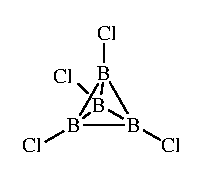
\includegraphics{picture/B4Cl4.eps}
        \end{minipage}
    }
    \subfigure[\ce{B8Cl8}的结构]{
        \begin{minipage}[b]{.3\linewidth}
            \centering\includegraphics{picture/B8Cl8.eps}
        \end{minipage}
    }
    \subfigure[\ce{B9Cl9}的结构]{
        \begin{minipage}[b]{.3\linewidth}
            \centering\includegraphics{picture/B9Cl9.eps}
        \end{minipage}
    }\caption{几种\ce{B_nCl_n}的结构}
\end{figure}
可以看到,它们的结构都和对应的\ce{[B_nH_n]^2-}相似,这是不符合Wade规则的又一例子.
\subsection{硼的含氧化合物}
硼(像硅一样)在自然界中总是以含氧化合物的形式存在,从来没有发现过单质硼或与其它非氧元素化合的硼\footnote{除了在意大利的Vesuvius火山口少量存在的氟硼钠石\ce{NaBF4}和氟硼钾铯石\ce{(K,Cs)BF4}.}.这些物质都具有复杂的结构,因此是一个值得探讨的内容.
\subsubsection{硼的氧化物}
\begin{substance}[\ce{B2O3}]
    三氧化二硼,化学式为\ce{B2O3},一般情况下为白色蜡状固体,但也可以形成为黑色玻璃态.\ce{B2O3}的熔点为$450\tc$,沸点为$1650\tc$.
\end{substance}
\ce{B2O3}是最难结晶的几种物质之一.它总是凝固形成玻璃态,而晶体$\alpha$-\ce{B2O3}则需要通过对无水\ce{H3BO3}小心加热脱水得到.无论何种形态,都以平面三角形的三配位\ce{\{BO3\}}单元为结构的基础,形成无限延伸的结构.
\begin{figure}[H]
    \subfigure[\ce{B2O3}的晶胞示意图]{
        \begin{minipage}[b]{.45\linewidth}
            \centering\includegraphics[scale=0.1]{picture/B2O3-1.eps}
        \end{minipage}
    }
    \subfigure[\ce{B2O3}的四倍晶胞示意图]{
        \begin{minipage}[b]{.45\linewidth}
            \centering\includegraphics[scale=0.1]{picture/B2O3-2.eps}
        \end{minipage}
    }\caption{\ce{B2O3}的晶体结构}
\end{figure}
气态的\ce{B2O3}以单体\ce{O=B-O-B=O}的形式存在.\\
\indent \ce{B2O3}作为酸性氧化物和各种金属氧化物都能在熔融时化合生成具有鲜艳颜色的偏硼酸盐,并且颜色随着金属元素不同而不同.这就是著名的硼砂珠实验(实际操作可以直接加热硼砂与金属氧化物的混合物).\\
\indent \ce{B2O3}主要用于制造含硼玻璃.高硼硅玻璃的热膨胀系数更低,因此在冷却时受到的温度梯度应力更小,因此相比普通玻璃有更强的抗断裂性能.\\
\indent 将\ce{B2Cl4}水解即可得到\ce{B2(OH)4},然后再加热脱水即可得到硼的低氧化物\ce{(BO)_n}.这一物质在硼化物的制备中已经提到过.将硼单质与\ce{B2O3}共热亦可得到这种物质:
\begin{center}
    \ce{B2O3 + B -> 3BO}
\end{center}
因此,在过量硼单质存在的反应中,应当考虑这种物质的生成.
\subsubsection{硼的含氧酸}
\paragraph{硼酸\ce{H3BO3}}
\ce{H3BO3}是大多数硼化合物水解的最终正常产物,通常可由酸化硼砂的水溶液得到.
\begin{substance}[\ce{H3BO3}]
    硼酸,又称原硼酸,化学式为\ce{H3BO3}(写作\ce{B(OH)3}也许更合适).硼酸是白色粉末或片状白色透明晶体,在$169\tc$发生脱水生成偏硼酸.
\end{substance}
硼酸晶体中有着无限延伸的层状结构,层内的\ce{H3BO3}分子通过氢键相互连接,而层间距离则较大.这也解释了硼酸晶体的分层裂解性能和较低的密度.
\chemfig{H3BO3}{1}{\ce{H3BO3}的层状结构}
\indent 硼酸是一元弱酸,其酸性是通过接受\ce{OH-}而非电离出\ce{H+}实现的:
\begin{center}
    \ce{H3BO3 + 2H2O <=> H3O+ + [B(OH)4]-}\ \ \ $\text pK_\text a=9.25$
\end{center}
向硼酸水溶液中加入多羟基醇可以显著增强其酸性.形成螯合物在熵效应上占明显优势,因而能使平衡明显右移.
\begin{center}
    \ce{H3BO3 + 2Me2C(OH)C(OH)Me2 -> [B(Me2COCOMe2)2]- + H3O+ + 2H2O}\\
    \ce{H3BO3 + 2HOCH2C(OH)CH2OH -> [B(OCH2C(OH)CH2O)2]- + H3O+ + 2H2O}
\end{center}
生成的螯合离子的结构如下所示.
\begin{figure}[H]
    \subfigure[\ce{[B(Me2COCOMe2)2]-}的结构示意图]{
        \begin{minipage}[b]{.45\linewidth}
            \centering\includegraphics{picture/B(ORRO)2-1.eps}
        \end{minipage}
    }
    \subfigure[\ce{[B(OCH2C(OH)CH2O)2]-}的结构示意图]{
        \begin{minipage}[b]{.45\linewidth}
            \centering\includegraphics{picture/B(ORRO)2-2.eps}
        \end{minipage}
    }\caption{硼酸多羟基醇酯阴离子的结构}
\end{figure}
我们在介绍浓硫酸的性质时已经说过\ce{H3BO3}在硫酸中生成\ce{[B(HSO4)4]-},因而表现得像强酸:
\begin{center}
    \ce{H3BO3 + 6H2SO4 -> 3H3O+ + 2HSO4- + [B(HSO4)4]-}
\end{center}
硼酸与\ce{ROH/H2SO4}反应即可得到对应的硼酸酯\ce{B(OR)3}.它与\ce{H2O2}也可以反应得到过一硼酸盐\ce{[HOOB(OH)3]-}和过硼酸盐\ce{[B2(OH)4(O2)2]^2-},结构分别如下:
\begin{figure}[H]
    \subfigure[\ce{[HOOB(OH)3]-}的结构示意图]{
        \begin{minipage}[b]{.45\linewidth}
            \centering\includegraphics{picture/HOOB(OH)3-.eps}
        \end{minipage}
    }
    \subfigure[\ce{[B2(OH)4(O2)2]^2-}的结构示意图]{
        \begin{minipage}[b]{.45\linewidth}
            \centering\includegraphics{picture/B2(OH)4(O2)22-.eps}
        \end{minipage}
    }\caption{过氧硼酸根的结构}
\end{figure}
\paragraph{偏硼酸\ce{HBO2}}
加热硼酸使其部分脱水即可得到偏硼酸\ce{HBO2}.正交\ce{HBO2}中存在其三聚体\ce{B3O3(OH)3},其层状结构如下:
\chemfig{HBO2}{1}{正交\ce{HBO2}的层状结构}
因此也可以看出,具有$C_3$轴的\ce{B3O3(OH)3}是更稳定的构象异构体.
\subsubsection{硼酸盐}
\paragraph{硼酸盐结构综述}
大体而言,硼酸盐中的\ce{B}总是平面三角形构型或四面体构型的.我们把一些典型硼酸盐的阴离子结构和对应的盐给出如下.
\begin{figure}[H]
    \centering
    \subfigure[\ce{[BO3]^3-} \ce{Mg3(BO3)2,LaBO3}]{
        \begin{minipage}[b]{.23\linewidth}
            \centering\includegraphics{picture/BO33-.eps}
        \end{minipage}
    }
    \subfigure[\ce{[B2O5]^4-} \ce{Mg2B2O5,Fe2B2O5}]{
        \begin{minipage}[b]{.23\linewidth}
            \centering\includegraphics{picture/B2O54-.eps}
        \end{minipage}
    }
    \subfigure[\ce{[B3O6]^3-} \ce{K3B3O6,BaB2O4}]{
        \begin{minipage}[b]{.23\linewidth}
            \centering\includegraphics{picture/B3O63-.eps}
        \end{minipage}
    }
    \subfigure[\ce{[BO2]^{n-}_n} \ce{Ca(BO2)2}]{
        \begin{minipage}[b]{.23\linewidth}
            \centering\includegraphics{picture/BO2-.eps}
        \end{minipage}
    }\caption{硼酸盐阴离子的结构I$-$平面三角形配位的硼酸根阴离子}
\end{figure}
\begin{figure}[H]
    \centering
    \subfigure[\ce{[BO4]^5-} \ce{TaBO4}]{
        \begin{minipage}[b]{.4\linewidth}
            \centering\includegraphics{picture/BO45-.eps}
        \end{minipage}
    }
    \subfigure[\ce{[B(OH)4]-} \ce{Na[B(OH)4]}]{
        \begin{minipage}[b]{.4\linewidth}
            \centering\includegraphics{picture/B(OH)4-.eps}
        \end{minipage}
    }
    \subfigure[\ce{[B2O(OH)6]^2-} \ce{Mg[B2O(OH)6]}]{
        \begin{minipage}[b]{.4\linewidth}
            \centering\includegraphics{picture/B2O(OH)62-.eps}
        \end{minipage}
    }
    \subfigure[\ce{[B2(OH)4(O2)2]^2-} \ce{NaBO3.4H2O}]{
        \begin{minipage}[b]{.4\linewidth}
            \centering\includegraphics{picture/B2(OH)4(O2)22-.eps}
        \end{minipage}
    }\caption{硼酸盐阴离子的结构II$-$四面体配位的硼酸根阴离子}
\end{figure}
\begin{figure}[H]
    \centering
    \subfigure[\ce{[B5O6(OH)4]-} \ce{K[B5O6(OH)4].2H2O}]{
        \begin{minipage}[b]{.3\linewidth}
            \centering\includegraphics{picture/B5O6(OH)4-.eps}
        \end{minipage}
    }
    \subfigure[\ce{[B3O3(OH)5]^2-} \ce{Ca[B3O3(OH)5].H2O}]{
        \begin{minipage}[b]{.3\linewidth}
            \centering\includegraphics{picture/B3O3(OH)52-.eps}
        \end{minipage}
    }
    \subfigure[\ce{[B4O5(OH)4]^2-} \ce{Na2[B4O5(OH)4].8H2O}]{
        \begin{minipage}[b]{.3\linewidth}
            \centering\includegraphics{picture/B4O5(OH4)2--1.eps}
        \end{minipage}
    }\caption{硼酸盐阴离子的结构III$-$兼有三配位和四配位硼的硼酸根阴离子}
\end{figure}
\paragraph{硼砂}
作为一种使用历史悠久的矿物,有关硼砂有很多值得了解的内容.
\begin{substance}[\ce{Na2B4O7.10H2O}]
    硼砂(Borax),化学式为\ce{Na2B4O7.10H2O},为质地较软的白色粉末或无色晶体.硼砂略带甜味和咸味,易溶于水,置于空气中则容易失去结晶水而风化.硼砂有一定毒性,摄入可能导致肝肾功能受损和内分泌紊乱.
\end{substance}
\subparagraph{硼砂的历史}
中国是最早发现和使用硼砂的国家之一.这种盛产于西藏,青海\footnote{据说有人在某年初赛时看到青海湖就推出了硼砂.}等地的矿物最初被用作金属助焊剂,因而硼砂最初被称作\tbf{焊剂}(tincal).在公元8世纪,源自西藏,波斯和亚洲其它地区的天然硼砂通过丝绸之路被运往西方.硼砂的英文名Borax则可能来源于波斯语Burah,意为“白色闪亮的矿物”.
\subparagraph{硼砂的结构}
虽然硼砂经常地被写作\ce{Na2B4O7.10H2O},但事实上其中的阴离子为\ce{[B4O5(OH)4]^2-}.晶体中的离子通过氢键连接形成长链.\ce{Na+}被\ce{H2O}六配位而形成八面体,八面体共边连接形成另一种长链.两种长链通过氢键连接,作用力相对较弱,因而硼砂晶体质地较软.
\begin{figure}[H]
    \centering
    \subfigure[\ce{[B4O5(OH4)]^2-}离子的立体结构示意图]{
        \begin{minipage}[b]{.33\linewidth}
            \centering\includegraphics{picture/B4O5(OH4)2--2.eps}
        \end{minipage}
    }
    \subfigure[硼砂中\ce{[B4O5(OH4)]^2-}形成的长链]{
        \begin{minipage}[b]{.63\linewidth}
            \centering\includegraphics{picture/B4O5(OH4)2--3.eps}
        \end{minipage}
    }\caption{硼砂的相关结构}
\end{figure}
\subparagraph{硼砂的化学性质}
硼砂容易失水.加热到$75\tc$,即失水得到\ce{NaB4O7.5H2O},再加热到$200\tc$即得到\ce{Na2B4O7},即无水硼砂.无水硼砂中并没有分立的\ce{[B4O7]^2-},而是形成复杂的网状结构.\\
\indent 硼砂水溶液是天然的缓冲溶液.这是因为\ce{[B4O5(OH)4]^2-}水解的方式如下:
\begin{center}
    \ce{[B4O5(OH)4]^2- + 5H2O -> 2[B(OH)4]- + 2B(OH)3}
\end{center}
恰好产生比例为$1:1$的硼酸和硼酸阴离子,形成缓冲对.
\paragraph{含\ce{B-O}键的有机化合物}
硼酸酯大多含有三配位的硼.\\
\indent 最简单的三硼酸酯\ce{B(OMe)3}可以由\ce{B2O3}或\ce{H3BO3}与\ce{MeOH}反应得到.它燃烧时产生的特征绿色火焰是鉴定\ce{B}元素的一种手段.\\
\indent 对\ce{H3BO3}的不完全烷基化可以得到\ce{RB(OH)2}.它可以脱水三聚形成含有\ce{B-O}六元环的\ce{B3O3R3},其结构与\ce{HBO2}的三聚体相似.
\subsection{硼氮化合物}
\paragraph{氮化硼\ce{BN}}
氮化硼的概述如下.
\begin{substance}[\ce{BN}]
    氮化硼,化学式为\ce{BN}.六方$\alpha$-\ce{BN}又称白石墨,是白色固体.立方$\beta$-\ce{BN}是类似金刚石的固体,为无色到琥珀色的极坚硬的固体.
\end{substance}
\subparagraph{\ce{BN}的制备}
制备\ce{BN}有很多技术困难.实验室通常采用熔融硼砂和氯化铵的混合物:
\begin{center}
    \ce{Na2B4O7.10H2O + 4NH4Cl ->T[熔融] 2NaCl + 2HCl + 17H2O + 4BN}
\end{center}
工业上大规模的合成可以采取硼酸与尿素在\ce{NH3}气氛中共热得到:
\begin{center}
    \ce{2H3BO3 + 6CO(NH2)2 ->T[熔融][\ce{NH3}] 2BN + 6CO2 + 10NH3}
\end{center}
“只有勇敢的或十足傻瓜的化学家才企图写出这两个反应的配平的方程式.”\footnote{N. N. Greenwood, A. Earnshaw. 元素化学[M]. 北京:高等教育出版社, 1997.}尽管Greenwood如此写道,但笔者认为配平这两个方程式仍是应当掌握的知识.另外一种方式是将\ce{NH3}与\ce{BF3}反应的产物\ce{H3NBF3}加热:
\begin{center}
    \ce{4H3NBF3 ->T[$\Delta$] 3NH4BF4 + BN}
\end{center}
\subparagraph{\ce{BN}的结构}
六方$\alpha$-\ce{BN}的结构与石墨大体上比较相似,是由\ce{B-N}六元环构成的平面结构堆叠而成.然而不同的是,石墨中的各层是交错重叠的(这也衍生出了三方石墨和六方石墨两种晶型),而六方$\alpha$-\ce{BN}的两层是完全重叠的,每个\ce{B}原子与上下两层的\ce{N}原子在投影上对齐.这可能是静电相互作用导致的.此外,其中的\ce{B-N}键键长为$135\text{ pm}$,明显短于正常的\ce{B-N}键,因此说明其有明显的$\pi$键性质.
\chemfig{alpha-BN}{0.1}{六方$\alpha$-\ce{BN}的晶胞}
六方$\alpha$-\ce{BN}因其层状结构和较弱的层间作用力而可以作为优良的润滑剂.\\
\indent 在高温高压下,六方$\alpha$-\ce{BN}可以转化为闪锌矿型的立方$\beta$-\ce{BN}或纤锌矿型的六方$\beta$-\ce{BN}.
\subparagraph{\ce{BN}的性质与反应}
尽管六方$\alpha$-\ce{BN}键长平均化,但它并不像石墨一样非常稳定.在氟化氢的作用下,\ce{BN}可以转化为\ce{NH4BF4},而氟气则定量地使其转化为\ce{N2}和\ce{BF3}:
\begin{center}
    \ce{BN + 4HF -> NH4BF4}\\
    \ce{2BN + 3F2 -> 2BF3 + N2}
\end{center}

\indent 六方$\alpha$-\ce{BN}也可以作为优良的绝缘体.\\
\indent $\beta$-\ce{BN}则和金刚石类似,具有优良的硬度和绝缘性,常常被用作磨料和刀具头.
\paragraph{胺-硼烷加合物\ce{R3NBX3}和氨硼烷\ce{R2NBX2}}
最简单的此类配合物\ce{H3NBH3}并不能由\ce{NH3}与\ce{B2H6}的反应得到.前面已经说过,这将发生不对称裂解,因此需要换一种方法制备:
\begin{center}
    \ce{2NH3 + B2H6 -> [(H3N)2BH2]+[BH4]-}\\
    \ce{LiBH4 + NH4Cl -> H3NBH3 + H2 + LiCl}
\end{center}
其它氨硼烷或类似物,大多可以采用直接化合的方式得到,例如\ce{H3NBF3},\ce{Me3NBH3}等等.\\
\indent 尽管这些配合物中\ce{N}带形式正电荷,\ce{B}带形式负电荷,但事实上\ce{N}的配位并不能改变\ce{B}的正电性.亲核试剂仍然会进攻\ce{B}.
\indent 氨硼烷\ce{R2NBX2}也有类似的性质.尽管我们可以写出含有\ce{B=N}双键的(键长数据也支持此结论),\ce{N}带形式正电荷而\ce{B}带形式负电荷的共振式,但体现亲电性的仍然是\ce{B}原子(这就和羰基是类似的).例如,\ce{H2BNMe2}容易发生二聚,产物\ce{[H2BNMe2]2}的结构如下所示.
\chemfig{[H2BNMe2]2}{1}{\ce{[H2BNMe2]2}的结构}
\paragraph{无机苯\ce{B3N3H6}}
无机苯是环氮硼烷中最重要的一类.最初,Alfred Stock和Erich Pohland通过乙硼烷与氨的反应合成了无机苯:
\begin{center}
    \ce{3B2H6 + 6NH3 ->T[$180\tc$] 2B3N3H6 + 12H2}
\end{center}
采用\ce{NaBH4}还原\ce{(NH4)2SO4}亦可:
\begin{center}
    \ce{6NaBH4 + 3(NH4)2SO4 -> 2B3N3H6 + 3Na2SO4 + 18H2}
\end{center}
此外,还可以用两步法制备:
\begin{center}
    \ce{3BCl3 + 3NH4Cl -> B3Cl3N3H3 + 9HCl}\\
    \ce{2B3Cl3N3H3 + 6NaBH4 -> 2B3N3H6 + 3B2H6 + 6NaCl}
\end{center}
作为苯的等电子体,无机苯\ce{B3N3H6}尽管是平面结构且有着等长的\ce{B-N}键,其环电流却似乎十分微弱,并没有显现出明显的芳香性.它容易与\ce{H2O,ROH,HX}等物质反应生成$1:3$的加合物,加热后又容易失去\ce{H2}而重新变为平面型分子,只是\ce{B}上的基团被替换:
\begin{center}
    \ce{B3N3H6 + 3H2O ->T[$0\tc$] [BH(OH)NH2]3}\\
    \ce{[BH(OH)NH2]3 ->T[$100\tc$] B3(OH)3NH3 + 3H2}
\end{center}
\subsection{硼的其他化合物}
\paragraph{硼的硫化物}
在尝试合成硫代硼酸的过程中得到了\ce{HSB2},主要以二聚体和三聚体的形式存在,其结构分别如下:
\begin{figure}[H]
    \centering
    \subfigure[\ce{(HBS2)2}]{
        \begin{minipage}[b]{.4\linewidth}
            \centering\includegraphics{picture/(HBS2)2.eps}
        \end{minipage}
    }
    \subfigure[\ce{(HSB2)3}]{
        \begin{minipage}[b]{.4\linewidth}
            \centering\includegraphics{picture/(HBS2)3.eps}
        \end{minipage}
    }\caption{硫代偏硼酸的结构}
\end{figure}
\indent 硼单质和硫单质混合加热即可得到最简式为\ce{BS2}的化合物,其中实际上含有类似卟吩大环结构.
\chemfig{B8S16}{1}{\ce{B8S16}的结构}
你可以尝试写出它的共振式\footnote{这就是第35届中国化学奥林匹克初赛第3题的最后一问.}.
\end{document}